\section{Earlier Action-Advising and Execution Comparisons}
\label{sec:supp:earlier}

Before the conditional-bank experiments, we investigated selective
action advising. These studies have different training horizons,
cohorts and supervision procedures from the main bank study. We
report their within-study comparisons separately. This section also
reports action-execution variants and their evaluation protocols.

\subsection{Selective online action advising}
An earlier MultiRoom-N6 study compares no advice, entropy-based query
selection, probability correction at threshold .20, and uniform random
query times. The teacher is GPT-5-mini with full-map access; recommended
actions supply cross-entropy targets while the student chooses its own
actions. The study uses five paired seeds, recurrent PPO or Count-PPO,
9,999,360 transitions, an initial imitation coefficient of 1.0 and a maximum
of 480 consultations per guided run. These settings differ from the
current bank study and from its request-matched online comparison.



All plain-PPO evaluation curves remain at zero in this cohort. Count-PPO
mean AUC is .348 without advice, .989 with entropy, .992 with probability
correction, and .945 with random queries. Probability correction delivers
127.2 labels per run on average versus 428.8 for entropy, while each uses
480 consultations. This demonstrates the distinction between delivered
labels and teacher queries. These procedures retain an inherited
random-number coupling between advice scheduling and PPO updates, identified
in a later audit; effects should be attributed to the tested procedures
rather than solely to the semantic content of received labels.

\subsection{Learning curves and the meaning of mistake correction}
Probability correction delivers a usable teacher target $a^T$ only when
$\pi_\theta(a^T\mid x)<0.2$, following the entropy-based query mechanism.
Exact-disagreement correction, explored in other earlier studies, instead
requires disagreement between the sampled student action and the teacher
action. Neither criterion proves that the teacher is correct. Random
query times choose when to request advice; they do not replace environment
actions with random actions. The online advisor controls teaching
opportunities or delivery, while the conditional bank controls the
applicability of reusable recommendations.

For the earlier MultiRoom study, probability correction and entropy
selection both use 480 consultations per Count-PPO run, but deliver means
of 127.2 and 428.8 labels, respectively. Neither pre-specified advisor
contrast establishes superiority after its family adjustment, and similar
mean performance is not an equivalence result. The same procedures leave
plain PPO at zero observed success. Timing, delivered dose and the inherited
random-number coupling also differ; these are comparisons of whole
procedures, not an isolated test of mistake detection.






\subsection{DoorKey advisors, importance and historical controls}
This section shows the complete earlier DoorKey and MultiRoom
online-advisor curves. DoorKey includes exact disagreement in addition
to entropy, probability correction and random query times. All three
entropy/correction plain-PPO arms have zero greedy AUC and final success.
Random queries reach 19.2\% final mean success, from one successful seed;
the no-advice mean is 3.6\%. Count-PPO reaches 100\% final mean success
with entropy, probability correction, random queries and no advice, and
80\% with exact disagreement. These results prevent describing every
earlier method as unsuccessful, while retaining their difficulty in
teaching plain PPO reliably in this cohort.

In a separate earlier DoorKey oracle screen, ten seeds per condition use
historical RGB observations, recurrent PPO without count bonus and 10M
transitions. Every guided arm delivers 200 labels. Teacher-Q importance
uses $\max_a Q_T(s,a)-\min_a Q_T(s,a)$; top-two-gap importance uses one
minus the gap between the student's two largest action probabilities;
entropy importance uses uncertainty across its action distribution.
Exact disagreement and probability-threshold correction apply additional
mistake criteria. Early advice supplies the initial labels without those
selection rules. These are a free oracle's labels, not LLM-generated rules.

All eight conditions have zero final greedy success. Sampled final means
range from 1.0\% without advice to 14.2\% for exact disagreement.
Figure~\ref{fig:legacy_importance} shows both metrics. Only final recorded
evaluations are used here; training-episode rewards are not substituted
for teacher-free evaluation curves. Seeds 0--4 and 5--9 use two recorded
source revisions, retained as historical blocks. These results do not
establish a general ranking of importance criteria or a matched
comparison with our current symbolic-observation bank study.

\begin{figure}[htbp]\centering
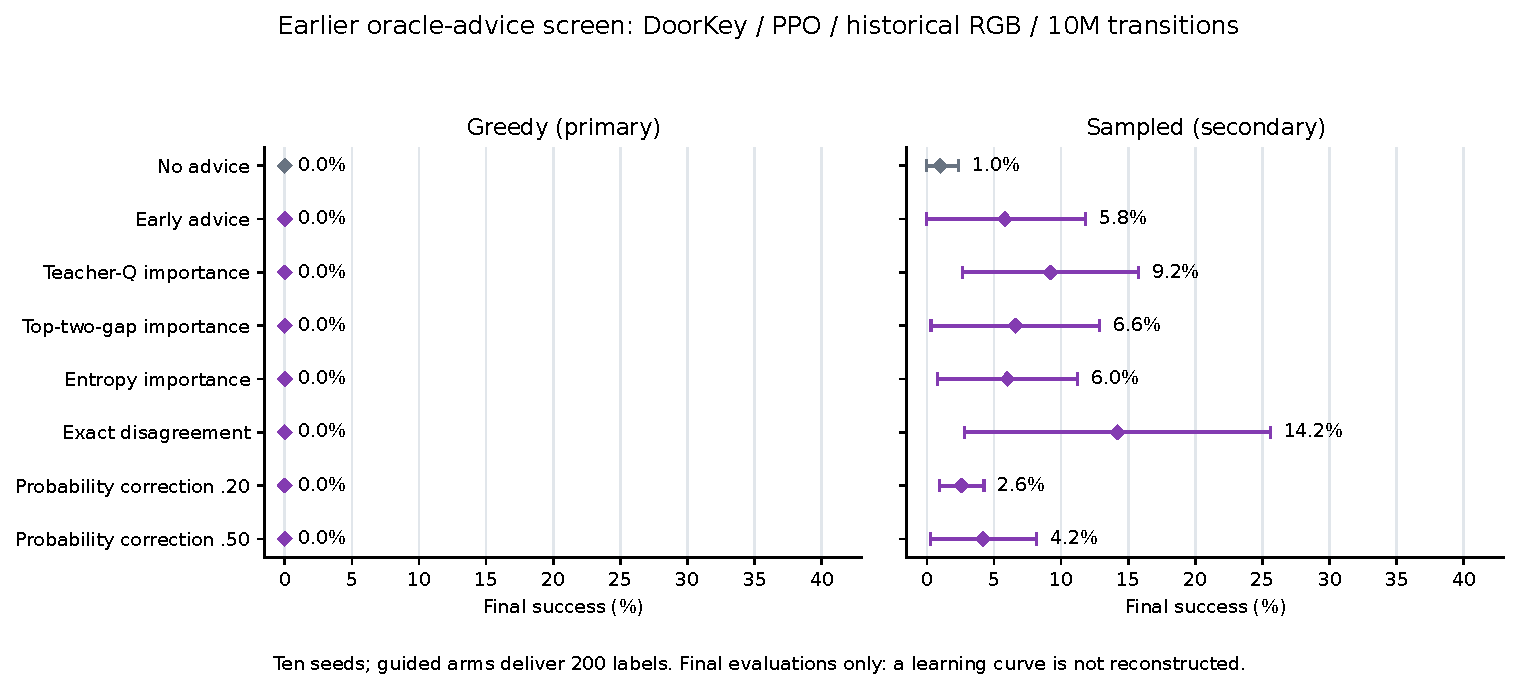
\includegraphics[width=\linewidth]{figures/legacy_importance_endpoints.pdf}
\caption{Historical oracle-advice screen: final teacher-free evaluation
of eight procedures, ten training seeds each, 10M transitions and 200
labels per guided run. Left: primary greedy success. Right: secondary
sampled success. Points are means with unadjusted 95\% $t$-intervals over
training seeds, clipped to the feasible range for display. The different
observation representation, teacher and code-revision blocks remain
explicit; this is not a current-bank baseline.}
\label{fig:legacy_importance}
\end{figure}

\subsection{Execution variants and evaluation comparability}
The current same-bank execution variant intermittently replaces the
student's action with the rule target while retaining the imitation loss.
The only non-identifier argument changes against the paired label-only
configuration are the execution start probability (0.75) and schedule
fraction (0.5). The probability is
$0.75\,0.01^{f/0.5}$ at training fraction $f$, until advice ends at $f=0.75$.
Its mixed behavior policy is scored using student-policy probabilities
in PPO. This known formulation limitation remains part of the reported
procedure. It is not the RLingua-style A/B implementation, which handles
controller transitions separately.

The same-bank comparison does not show that action execution is generally
unsuccessful. For example, it has mean greedy AUC 0.896 on KeyCorridor PPO,
versus 0.733 for label-only teaching; the paired contrast is inconclusive
after correction. Label-only teaching meets the declared 0.05 AUC
non-inferiority margin in five of the six settings. Figure~\ref{fig:execution_sampled}
adds sampled evaluation of the same trained students; primary paired
claims remain based on greedy AUC.

\begin{figure}[htbp]\centering
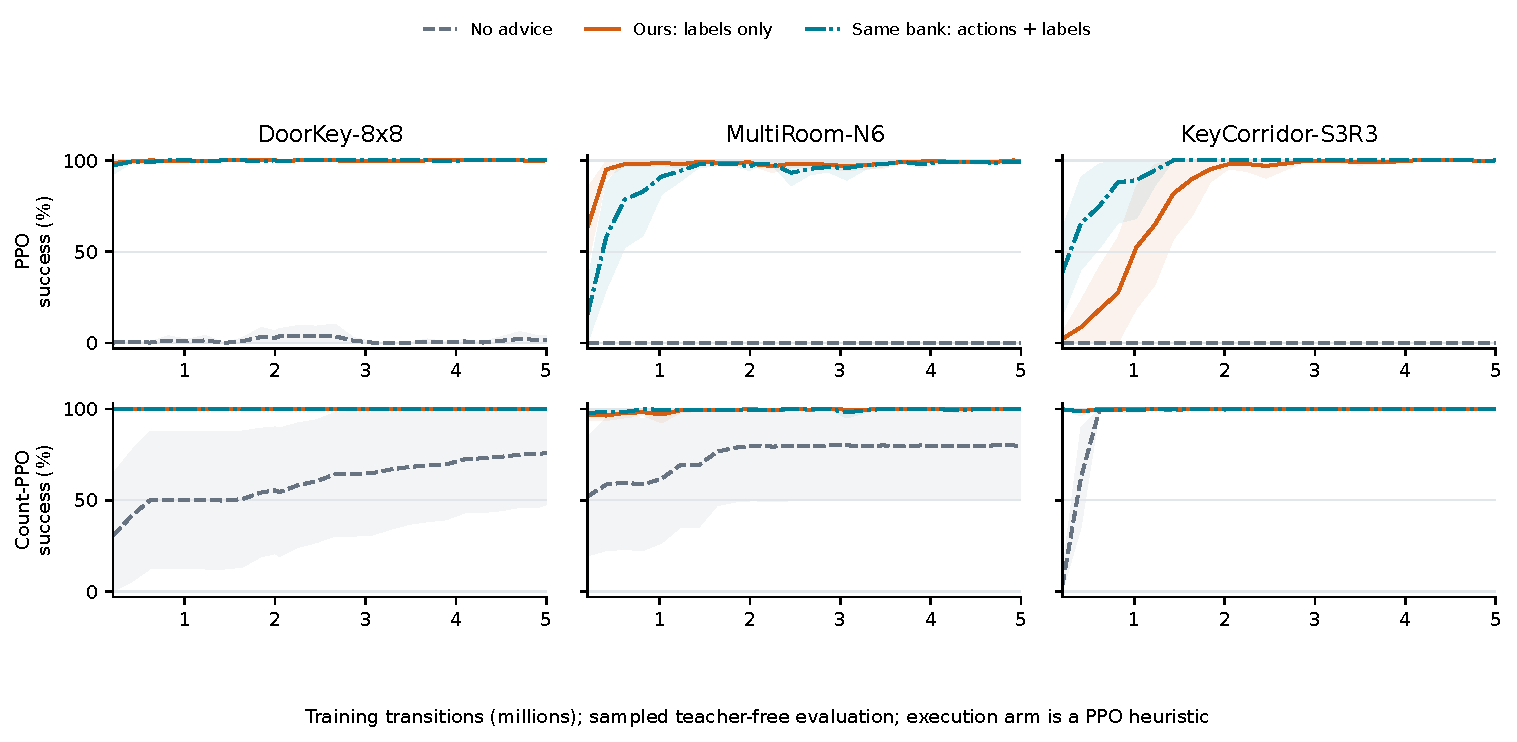
\includegraphics[width=\linewidth]{figures/bank_execution_sampled.pdf}
\caption{Secondary sampled-action evaluation of the same-bank teaching
comparison. Students and checkpoints match the greedy execution comparison below;
ten paired training seeds per task--student setting and 5M transitions.
Teaching is disabled during evaluation. Bands are pointwise 95\%
$t$-intervals clipped for display. The execution heuristic retains its
probability-accounting limitation.}
\label{fig:execution_sampled}
\end{figure}

Earlier override and teacher-prefix pilots are retained as historical
method-development records. Their channel comparisons used different
teacher-off measurements: dedicated greedy evaluation for distillation,
but recent stochastic training success after teacher removal for the
other channels. These quantities are not combined into a matched
performance plot. The present same-bank and A/B comparisons provide the
clearer action-execution evidence for the paper.


\begin{figure}[htbp]\centering
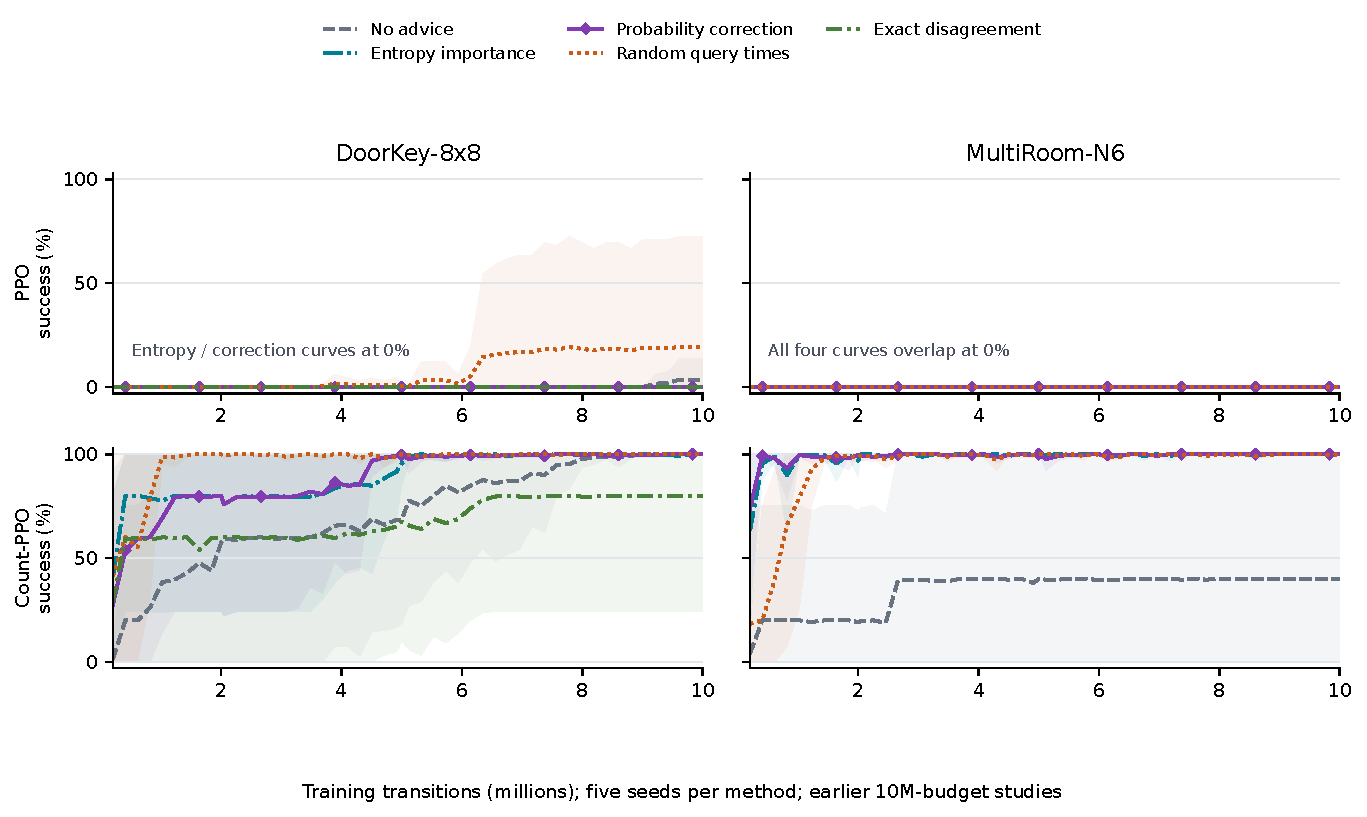
\includegraphics[width=\linewidth]{figures/earlier_online_advisors.pdf}
\caption{The earlier DoorKey and MultiRoom online-advisor studies, five
paired training seeds per method and 10M transitions. These are within-study
comparisons; cohorts and imitation settings differ from the current bank
study. Curves are mean greedy success with pointwise 95\% $t$-intervals.}
\end{figure}

\begin{figure}[htbp]\centering
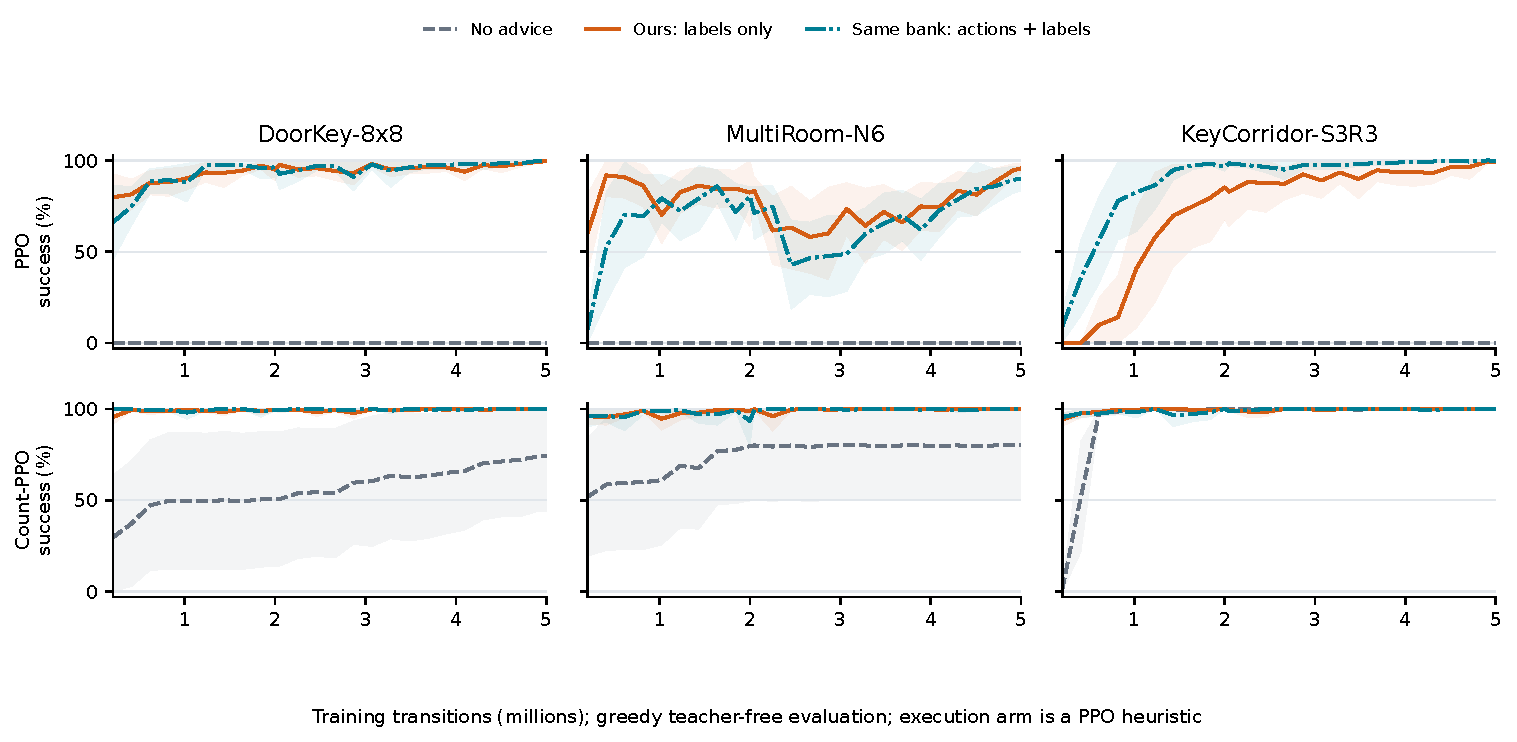
\includegraphics[width=\linewidth]{figures/bank_execution_greedy.pdf}
\caption{Same-bank greedy comparison of no advice, learning targets only,
and targets plus annealed action execution. Ten paired seeds per setting,
5M transitions, teacher-free evaluation. The execution variant retains
its known PPO probability-accounting limitation.}
\end{figure}
